\section{Discussion}


\subsection{Parameter Sensitivity}

\begin{itemize}
   \item[1.] \textbf{Sensitivity analysis of fragility against thresholds}

First, we try to fine-tune the demarcation point of the EPI and FSI index and calculate the average of the absolute values of residuals. It turns out that there is not a significant deviation in terms of fragility.
\begin{figure}[htbp]
    \centering
    \subfigure[Sensitivity against EPI]{
        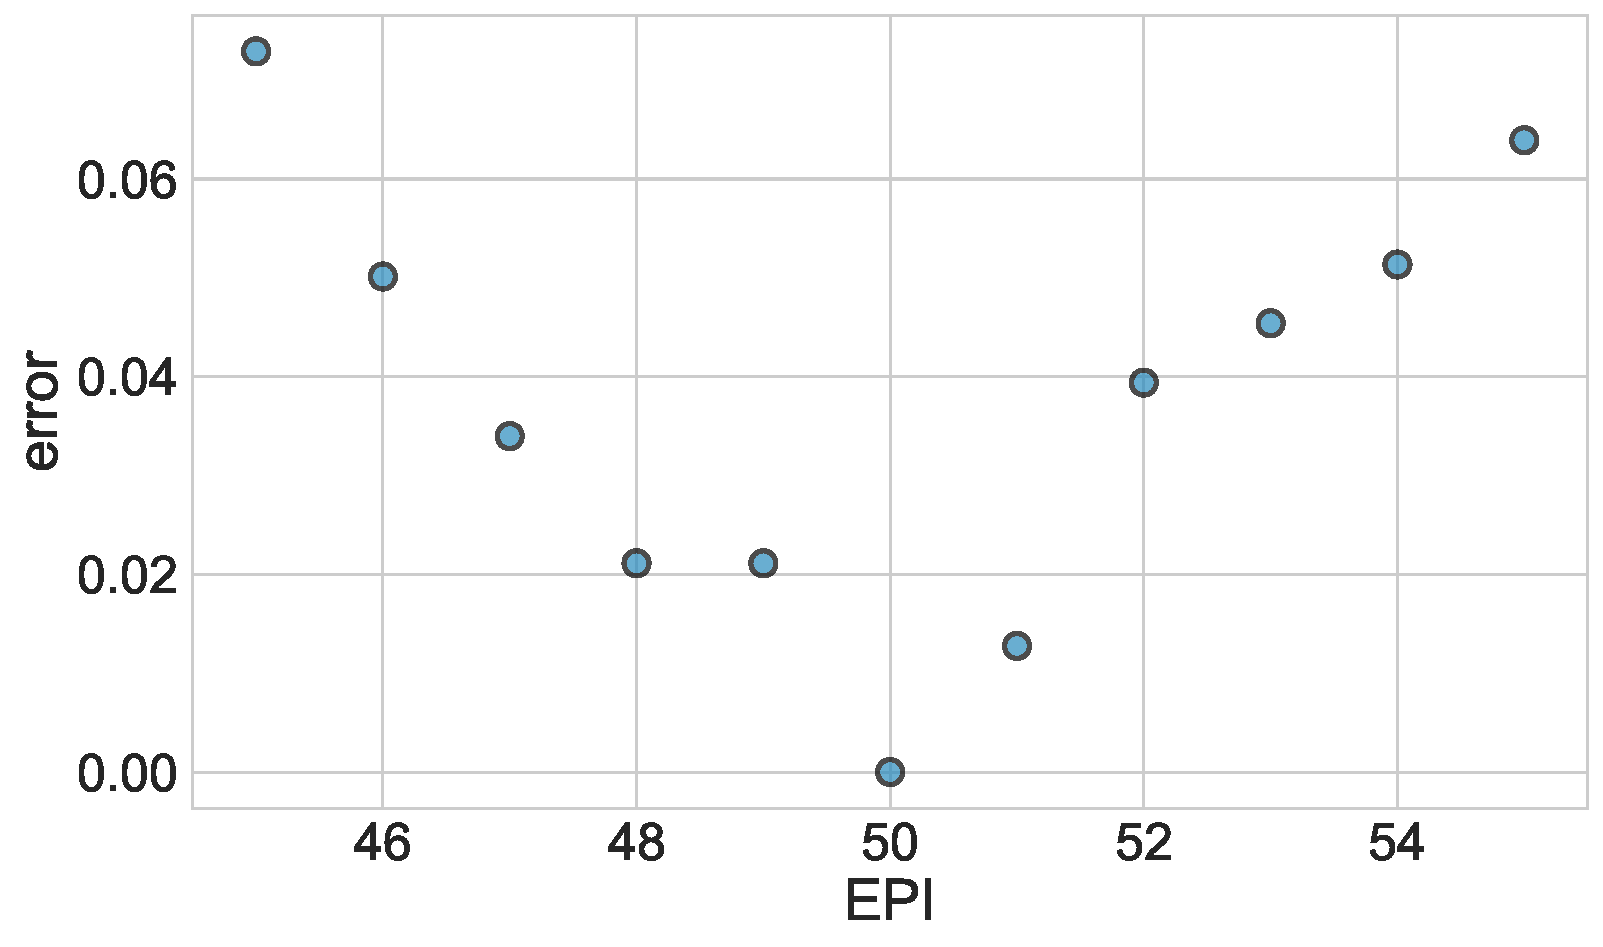
\includegraphics[width=.4\linewidth]{figs/error_EPI}
        \label{fig:exp:future:gdp}
    }
    \subfigure[Sensitivity against FSI]{
        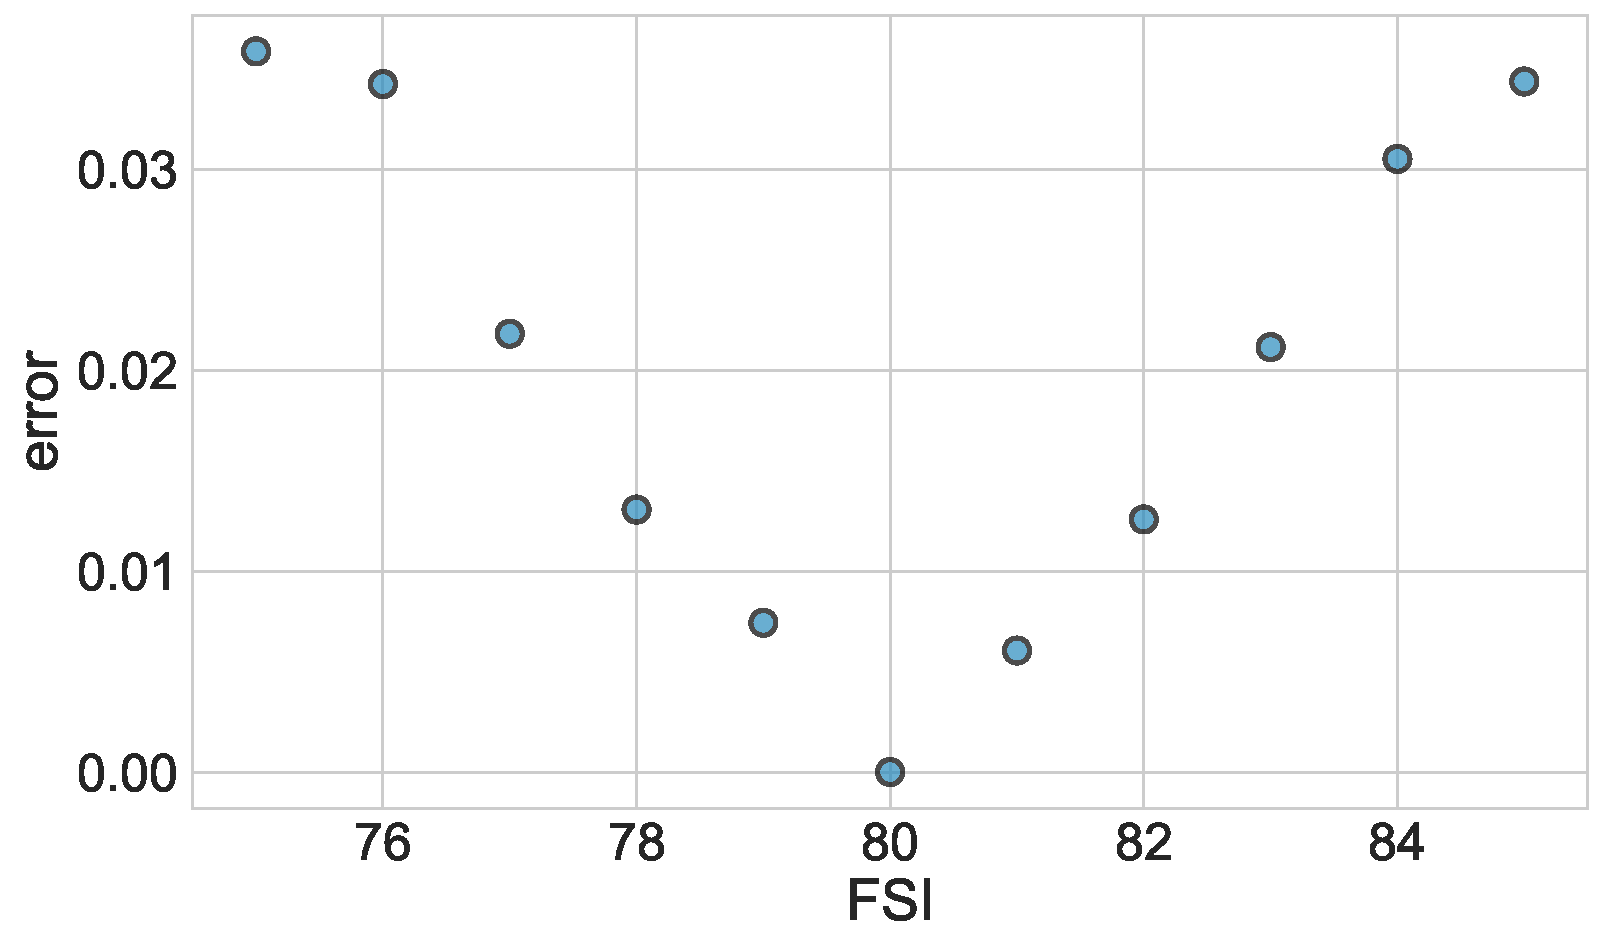
\includegraphics[width=.4\linewidth]{figs/error_FSI}
        \label{fig:exp:future:epi}
    }
    \caption{Fragility Sensitivity Analysis}
    \label{fig:exp:future}
\end{figure}
   \item[2.] \textbf{Predicted model sensitivity analysis}

Here we choose one country (Mauritius), the impact of the direct and indirect effects on the national fragile index are integrated. It is observed that there will not be a significant change in the predicted fragility when the EPI of the environmental index changes.
\begin{figure}[t]
    \centering
   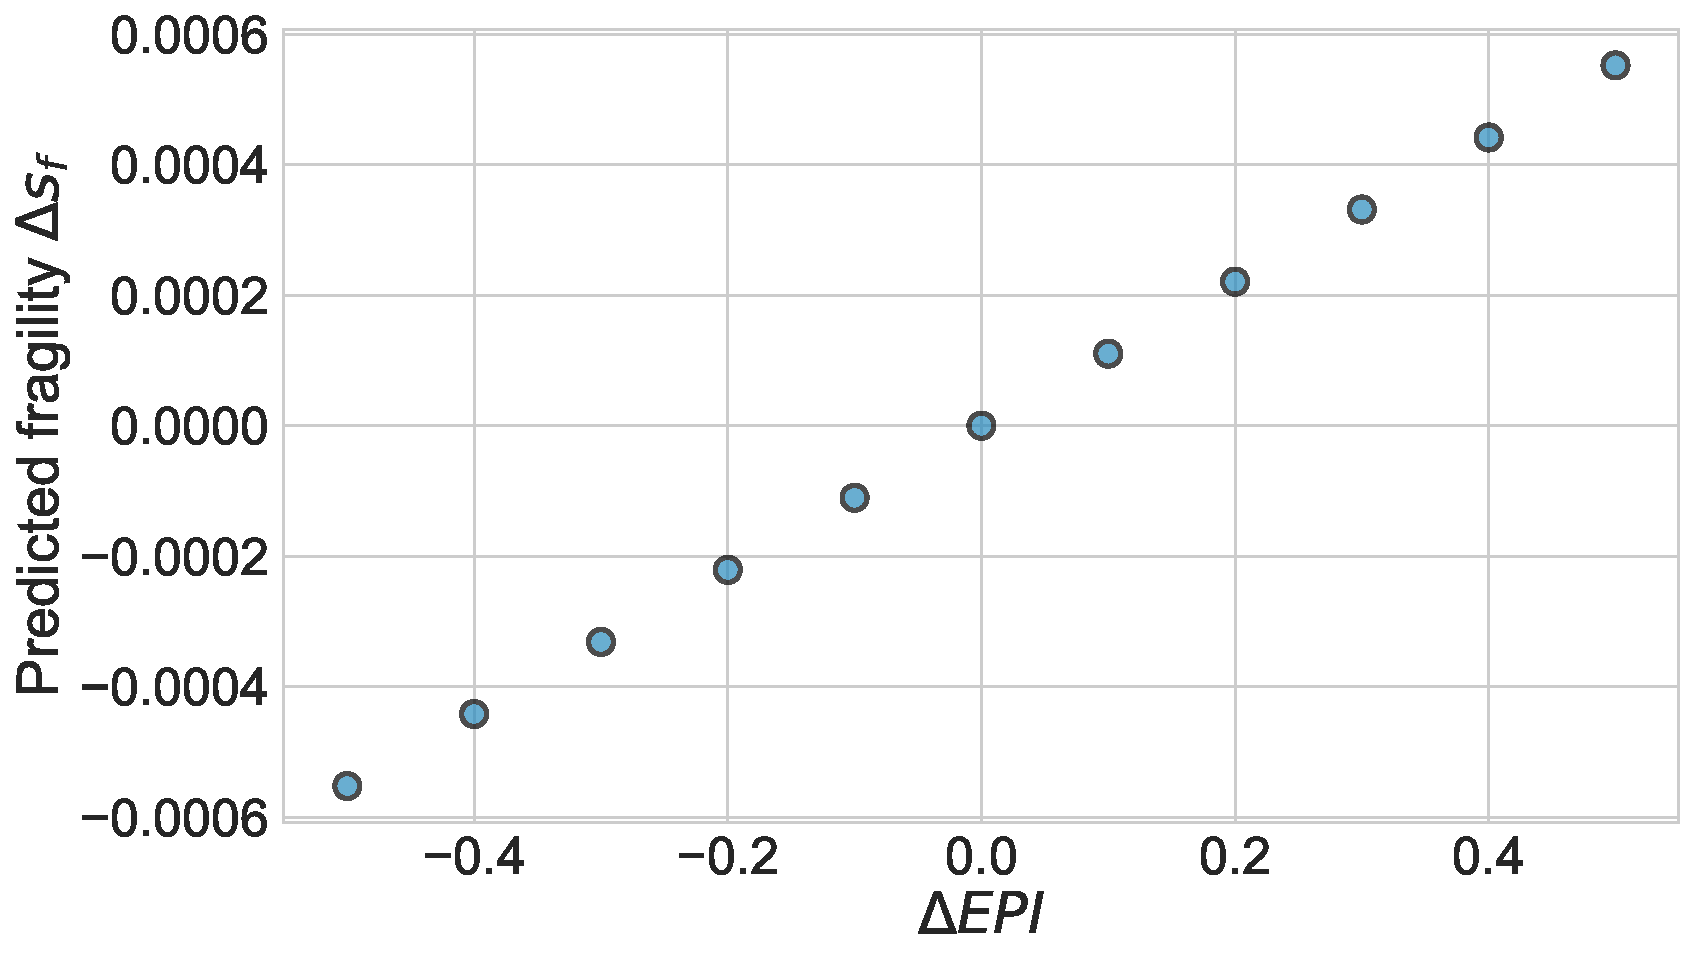
\includegraphics[width=.8\linewidth]{figs/predicted} 
   \caption{Predicted Fragility Sensitivity Analysis}
   \label{fig:model:model}
\end{figure}
   \item[3.] \textbf{Cross-validation for logistic regression}

When calculating the fragility, we use logistic regression to estimate probability. Here we test the accuracy of logistic regression with 5-fold cross-validation. The regression accuracy of different probability varies as the figure shows:
\end{itemize}

\subsection{Strength and Weakness}
We first give overall strength and weakness for our entire framework:
\begin{itemize}
   \item \textbf{Simplicity}. Our model is dedicated to capture the interaction between human and environmental factors in a simple, explainable, and verifiable fasion.
   \item \textbf{Objective}. Basic ideas are derived from convincing facts, while tools used to implement our ideas are theoretically well supported. Human error can be reduced to minimum. 
   \item \textbf{Flexibility}. Our theoretical framework applies to many scenarios other than countries and can be implemented in various methods. 
   \item \textbf{Appealing Results}. The result of our statistical analysis yields concrete conclusions consistent with interdisciplinary facts. The simulation results are convincing and insightful in finding the trade-off between fast economic growth and environment.
\end{itemize}

However, there are plenty of rooms for improvement for our model. 
\begin{itemize}
   \item Some hypothesis are too ideal. For example, we assumed that GDP is representative of human factors in the temporal model, and that EPI represents environmental fragility, without modeling the complex dynamics of climate change.
   \item Data limitation. Our simulation suffers from insufficient amount of data.
   \item Insufficient long-term prediction. Our long-term prediction of GDP and EPI used only recent information of a particular state and cannot well recognize complex dynamics in the long run.
\end{itemize}

\subsection{Extending the Model}

For smaller "states" such as cities, our theoretical framework still applies.
However, specific data preparation, variable selection, and model implementation should be modified accordingly. 
For larger "states" such as continents, our model is in need of describing the interactive relationship between countries to capture the evolution of the climate change and fragility of a organized whole, and its effect on each individual component state.

We give some analysis as follows:
\begin{itemize}
\item	External Intervention: 
It is one of elements given in the FSI index, which in turn plays an important role in our model. Here if we apply our model to figure out issues in terms of regions of various “scale”, there is no doubt that its influences will be significantly different. For example, cities of a country must have a closely connection with each other, while continents are not likely to be the same, or certainly not “that closely”.
One way to solve this problem is that we can set some systematic measures to represent it. Actually, we can even take it out to discuss its impact with FSI and EPI if necessary.
\item	Different Functions of Cities and National Conditions:
This is especially required to be considered when our model is applied to smaller “states”. Different Functions of cities means that fragility is not simply evaluated based on some indexes when it comes to smaller “states” issues. Instead, we are supposed to think over its function in this country. For example, some cities with better economy development or important political status may still not fragile although they have a terrible environment. Besides, different national condition will also affect the model, like different powers of government in every country.
To propose a better model, we may need to cluster different regions and describe the connection in every region more reasonably.
\item	Internal Difference of Continents:
Continents, to the contrary, are so few that there is little variety all over the world. However, if we would like to tell which continent is more fragile, it is necessary to distinguish its internal difference. For example, the fragility of different regions in Asia probably range a lot.
\end{itemize}

\hide{
As we analyzed above, our model requires to include a part to define what is the fragility of a large state, how it varies in different regions and how it influences the evaluation.
}

\subsection{Relation to Environmental Science}

\hide{
An Abrupt Climate Change Scenario and Its Implications for United States National Security (Peter Schwartz et al. 2003)
Is Climate Change a Driver of Armed Conflict? (Ole Magnus Theisen et al. 2013)
Modeling Environmental Security in Sub-Saharan Africa (Amy Richmond Krakowka et al. 2012)
}

Peter Schwartz et al. (2003) created an abrupt climate change scenario and analyzed its influence on United States National Security. Although its imagine was reasonable and meaningful for US society, the model was a little simple considering that it was one of pioneer works focusing on environmental security. Instead, our model pay more attention on the relation among human factors, environmental factors and fragility of states.

Like the former work, Ole Magnus Theisen et al. (2013) did research on the history of climate change and conflict occurrence. It contributed to linking climate change to conflict, and its methodology of linking elements is similar to our studies of correlation among independent factors. However, our model is interested in the whole framework of relation rather than some concrete climate changes.

Amy Richmond Krakowka et al. (2012) revealed the environmental security model in an Africa scenario. Its model mainly came from the relation among environment, security and conflict. With a process-outcome framework, it derived a specific conflict analysis, but our model concentrate on the global situation. Besides, we also consider the temporal model. In the process, we figure out how to take measures for the trade-off between economy development and environment protection.
